% Chapter 1

\chapter{The Problems with Solar} % Main chapter title

\label{Chapter1} % For referencing the chapter elsewhere, use \ref{Chapter1} 

\lhead{Chapter 1. \emph{The Problems with Solar}} % This is for the header on each page - perhaps a shortened title

%----------------------------------------------------------------------------------------
\section{Motivation}
The increasing demand for energy, combined with the surging interest in green technologies worldwide, has accelerated the need for a highly reliable, cost-efficient, and self-sustained electric power grid. Scientists and engineers everywhere agree without a shadow of a doubt that human power generation is the primary driver of the climate change phenomena wreaking havoc on our planet. Future energy distribution systems should be capable of interconnecting diverse power sources including fossil and nuclear-fueled generators, as well as renewable sources such as hydropower generators, wind turbines, and photovoltaic arrays. 

Renewable energy sources depend heavily on highly variable environmental conditions, and hence, require robust power conversion techniques that can handle unstable and highly varying input power\cite{ricardo}. The focus of this research-oriented senior design project has been to explore the viability and technical challenges involved with implementing new hybrid control techniques for solar power conversion. This research is of great interest to us, and the public in general, as it may prove to be a valuable addition to the power system designers toolkit for situations necessitating exceptionally clean output with robust stability characteristics in the face of highly variable load and source conditions.

We seek to understand the reported benefits of hybrid control techniques in the application of solar power converters. In particular, the conversion between the non-linear DC output of solar panels to steady AC power used in the power grid will be studied. In order to test the techniques which have been described analytically in \cite{ricardo}, the Hybrid Inverter Team, in partial fulfillment of the requirements for the Bachelors of Science in Electrical Engineering, will develop a small-scale power inverter capable of switching between pulse-width modulation and hybrid inverter algorithms. This development platform will allow for the straightforward comparison between the two. This report is intended to be an exhaustive account of our methodology and research in the pursuit of reaching these goals.

\section{Background}
In order to meet the challenge of building next-generation power conversion technologies capable of handling highly variable sources while simultaneously mitigating the problem of noise injection into the power grid, we must first understand the current landscape of power converters, analyze their strengths and weaknesses, and then assess how we might improve upon their implementations by leveraging today's inexpensive real-time microcontrollers, which have been tuned for power today's demanding power conversion applications. To this end, we will undertake a brief overview of the pulse-width modulation technique, the applicability of hybrid control algorithms to the problem of power conversion, and finally, we will briefly review the additional constraints that power conversion in the context of solar energy places on our design. 

\subsection{The Problems with Solar}
With the cost of photovoltaics rapidly decreasing, we have seen a rush toward the adoption of solar micro-grids which seek to exploit the most abundant source of power known to mankind - the sun. However, our heliocentric conundrum - namely the fact that the earth orbits the sun - dictates that most places on earth receive time-dependent quantities of solar irradiance over the course of any given day. This high variability in the context of power conversion implies major challenges to our modern power grid which guarantees nearly continuous up-time. Additionally, today's power conversion technologies are not robust to highly variable input sources like solar power. Some other challenges we face when converting DC solar power to AC power which is usable in our power grid is the problem of shading or partial irradiance of solar arrays, and the non-linear nature of the photovoltaics themselves. In particular, this non-linear behavior necessitates the implementation of maximum power point tracking or MPPT algorithms which comprehend this phenomena and harvest the most power from solar sources which typically have a finite lifespan. This is critical for obtaining the maximum benefit from the non-trivial investment required to operate solar arrays today. 

\subsection{Square and Modified Square Inverters}
Square wave inverters are the simplest method for generating pseudo-sinusoidal outputs using an H-Bridge. Emulating the positive and negative half cycles of the sine with a simple bipolar scheme where the output is given be $+V_{dc}$ and $-V_{dc}$ respectively. After a filtering stage, the output can be shaped into something resembling a sine wave by only allowing the low frequency components of the square wave to pass. Note that the difference between a pure square wave and a modified square wave is the allowance of the zero state determined by the quantity $\alpha$ shown in Figure \ref{modifiedSquare}. Note that the Fourier series of the output is given by 
\begin{equation}
v_0(t)=\sum\limits_{n,odd}V_n\sin{(n\omega_0t)}
\end{equation}
where 
\begin{equation}
V_n=\frac{4V_dc}{n\pi}cos{(n\alpha)}
\end{equation}
This would add considerably to the complexity of any inverter system seeking to control both parameters simultaneously. The harmonic content can be controlled by varying the quantity $\alpha$, and the amplitude can also be controlled by $\alpha$. With some analysis, it could be shown that the harmonic content or the amlpitude of the output can be controlled, but not both simultaneously unless we have a vairbale $V_{dc}$ input. 

\begin{figure}[h]
\centering
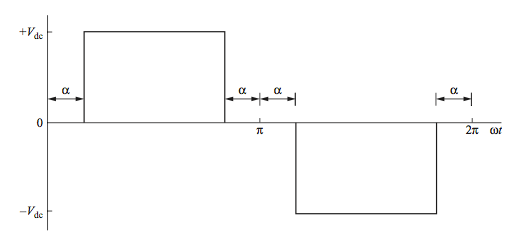
\includegraphics[width=3.5in]{modifiedSquare}
\caption{Modified Square Wave}
\label{modifiedSquare}
\end{figure}

The `deal-breaker' with the square wave inverter is the fact the the spectral content of the output is particularly rich at all odd harmonics of the fundamental. This means that we are left with a bulk of the harmonic content at low frequencies which are particularly hard to filter with analog components. 

\subsection{Linear Control and the PWM approach}
\label{pwmApproach}
Compared to square and modified square wave inverters, much of the filtering burden is alleviated due to the fact that spectral content in the vicinity of the fundamental is located near the frequency modulation index of the PWM signal. Pulse-width modulation (PWM), or bang-bang techniques, are a popular means for taking a fixed input voltage and varying the effective power seen at the output. This is done by rapidly switching the input off and on such that the the output is some fraction of the input including zero and one hundred percent. This fraction corresponds to the duty cycle. If we pair the PWM technique with the ability to drive current bidirectionally, say, through an H-Bridge circuit, we can use this technique to trace out a pseudo-sinusoidal output. 

In contrast to the square wave inverters discussed above, with PWM it is possible to vary amplitude and frequency independently. The modulation index, which is given by $m_f=\frac{f_{tri}}{f_{sin}}$ where $f_{tri}$ is the frequency of the triangular carrier frequency, and $f_{sin}$ is the sinusoidal reference signal. 

\begin{figure}[h]
\centering
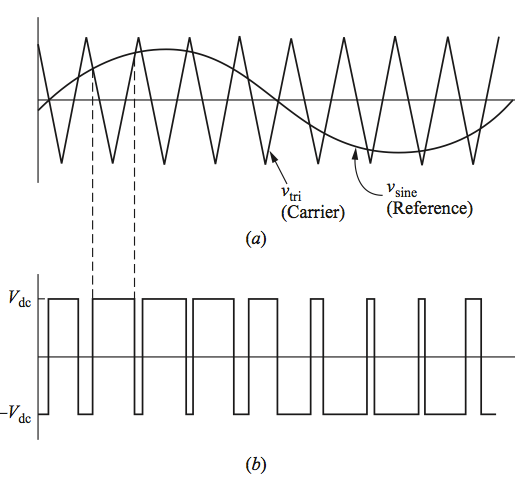
\includegraphics[width=3.5in]{bipolarSwitching}
\caption{Bipolar Switching}
\label{bipolar}
\end{figure}

The switch in this case can take the form of a relay, but more commonly in power applications, takes the form of a field-effect transistor (MOSFET) or insulated gate bipolar transistor (IGBT). The effective voltage or current is varied by varying the duration of on-time of the switch. One can think of this as int terms of a common household faucet with only two states, either fully on or off. If we were able to modulate the amount of time that the water flowed from the faucet, clearly we would be able to choose the flow-rate of the water from the two extrema - on or off - to an arbitrary level of precision depending on how fast we were able to turn the faucet on or off. The scenario put forth in the 'kitchen sink' analogy is analogous to the situation we face in a modern power inverter. In this case, we are faced with the challenge of taking a typically fixed input voltage and switching it in such a way that we achieve a close approximation to a sinusoidal output voltage. Given the clear explanation of how PWM techniques can vary from fully on to fully off in the description above, it is easy to see why the PWM approach has become the standard for power inverters. Additionally, today's microcontrollers have extremely sophisticated peripheral modules built specifically for very fast and PWM signal generation with resolution down to the nanosecond level becoming quite common. 

@todo:cite figures!
\begin{figure}[h]
\centering
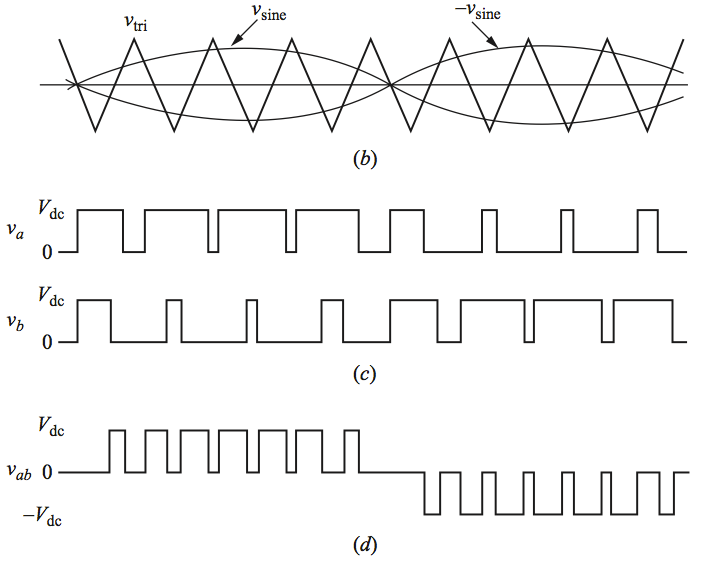
\includegraphics[width=3.5in]{unipolarSwitching}
\caption{Unipolar Switching}
\label{unipolar}
\end{figure}

The Fourier analysis for either bipolar or unipolar PWM output signals is not as straightforward as that of the square wave, so a full derivation is ommited from this discussion. However, the fact that the harmonic content occurs at multiples of the modulation frequency can be clearly observed in Figure \ref{pwmFourier}. 

\begin{figure}[h]
\centering
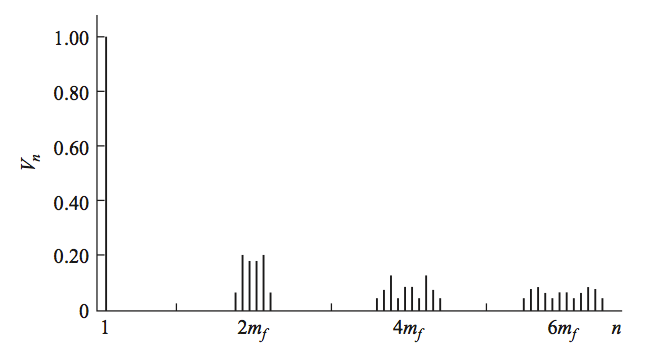
\includegraphics[width=3.5in]{pwmFourier}
\caption{Fourier Spectrum Frequency Diagram for PWM Inverter Control}
\label{pwmFourier}
\end{figure}

Although the PWM method for signal modulation has the clear advantages of widespread adoption and ease of implementation, with the widespread adoption of renewable energy in the form of highly local and decentralized micro-grids, we are increasingly faced with the problem of introducing increasing amounts of high-order noise into the power grid. Further, the typical proportional, integral, derivative, or PID methods for control suffer from a ringing phenomena in the presence of input disturbances which are typical of renewable energy applications. In light of these issues with the PWM technique for power conversion, we seek to explore alternate strategies for switching that might alleviate the vulnerability to  input disturbances and the problem of an unintentionally rich spectrum at the output of PWM power converters. 

\subsection{Hybrid Systems and Hybrid Control}
The study of hybrid systems has emerged in recent years as a response to the increasing entanglement of physical systems and computer control. 
Hybrid systems are those that exhibit both continuous and discrete-time dynamics. The system in question, namely the canonical power inverter topology, which is the focus of this research, is an excellent candidate for study under the lens of hybrid control due to the continuous evolution of a linear oscillator - our output filter - and the discrete time dynamics of the switch - in our case, a transistor receiving control signals from a micro. 

We seek to understand how hybrid control might alleviate some of the challenges associated with PWM techniques, a few of which have been outlined above. While a detailed explanation of the hybrid control algorithm is saved for later on in this paper, in a nutshell it has been found that with relatively simple physical models of our system, and the availability of discrete time switching, that we can generate outputs that closely resemble the desired sinusoidal outputs with less switching noise, and with a robust response to highly variable input voltages. For these reasons, we focus this research on the physical realization of such a hybrid system. One of the goals of this paper is to describe the algorithm designed by Jun Chai and Dr. Ricardo Sanfelice in more detail, and outline some of the challenges associated with realizing this implementation on a real world system \cite{ricardo}.

\section{Approach}
Switching power inverters are an enabling technology found in energy conversion systems. Photovoltaic (PV) panels harvest energy from the sun to generate the alternating current (AC) electricity used in the grid. PV arrays output direct current (DC) electricity, thus an inverter is required to generate the versatile AC power used in standard loads as shown in Figure~\ref{solarBlock}. Energy sourced from renewable resources is variable in nature and necessitates feedback controlled electronics to maintain stable power production.  This project is focused on delivering a microinverter system as a robust solution for solar power applications. 

Microinverter deployment strategies for solar systems offer improved reliability and reduced installation costs. Widespread integration of microinverters with individual solar panels to form AC power generation units removes single-point failure risks found in common centralized PV inverter arrangements. Microinverters for single panels can have longer mean times between failures since they are often designed for the 200W power range and operate with lower temperatures due to reduced heat waste. The economies of scale for manufacturing many consumer microinverters reduces hardware costs found in building few larger high power PV inverters.\cite{microchip} Another benefit of this microinverter approach is that the feedback control optimizes the power generation of all panels in the system to operate most efficiently considering each $unit's$ individual conditions. This makes them robust in situations like partial shading.

\begin{figure}
\centering
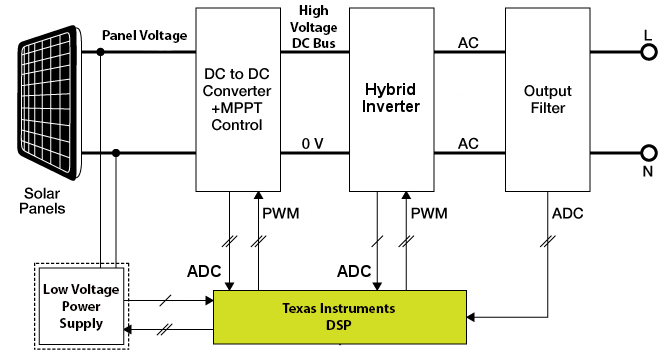
\includegraphics[width=3.5in]{solarBlockDiagram}
\caption{Inverter System Overview}
\label{solarBlock}
\end{figure}

Traditional inverters use a technique know as pulse width modulation (PWM) to generate AC power. This method is not as well adapted to input energy variation and also contributes some harmonic distortions to the output. A new hybrid systems based feedback control scheme for power switching is being utilized in this inverter as an alternative to PWM. AC output stability is achieved through comparison of real time measured voltages and currents compared to a defined reference sinusoid.\cite{ricardo} The hardware implementation  of a microinverter through this project will highlight the advantages of hybrid control to PWM.




